\chapter{Concepción y diseño de la solución}\label{chapter:solutionDesign}
En este capítulo se describe la concepción de la solución propuesta para el desarrollo 
del sistema destinado a la gestión de la información científica sobre las 
plantas medicinales cubanas, con base de conociemiento inicial en el libro de Tomás Roig. 
El capítulo está estructurado en tres secciones principales.

En primer lugar, se presenta el contexto en que se desarrolla la solución, 
explicando las motivaciones y necesidades que llevaron a su concepción. 
Posteriormente, se exponen los requerimientos que sirven como base de una modelación del problema, 
detallando cómo se definió y estructuró la problemática a resolver. 
Finalmente, se describe el diseño de la solución, dividida en dos subproblemas específicos, 
abordando el enfoque adoptado para dar respuesta a cada uno de ellos. 
Este análisis establece las bases conceptuales y técnicas necesarias para la 
posterior implementación y experimentación del sistema.



\section{Contexto del problema}
La iniciativa para desarrollar el presente sistema surge a partir de un diagnóstico 
conjunto realizado entre la Universidad de La Habana y el Jardín Botánico Nacional de Cuba, 
en el contexto de un acuerdo de colaboración científica. 
Este acuerdo tiene como objetivo principal la creación de soluciones que apoyen 
la preservación, organización y difusión del conocimiento botánico en el país, 
un campo que reviste gran importancia tanto para la investigación científica, 
como para la educación y el conociemiento general de las personas.

Durante este diagnóstico, se identificó que uno de los recursos más valiosos 
en el ámbito de la botánica cubana, el libro \textit{``Plantas medicinales, aromáticas o venenosas de Cuba''} 
de Tomás Roig y Mesa, enfrentaba múltiples desafíos relacionados con su accesibilidad y 
aprovechamiento. Este libro, publicado originalmente en 1945, constituye una obra 
de referencia fundamental que recopila una vasta cantidad de información científica 
sobre la flora medicinal de Cuba, incluyendo descripciones botánicas, 
usos terapéuticos y distribución geográfica de las plantas documentadas. 
Sin embargo, a pesar de su relevancia, el acceso a esta información sigue siendo 
limitado debido a varios factores:

\begin{itemize}
    \item \textbf{Formato físico predominantemente tradicional}: Aunque existen versiones 
    digitales del libro, estas no cuentan con un diseño modular que facilite su consulta 
    o análisis de la información. Esto reduce significativamente su usabilidad en contextos 
    modernos donde predominan las herramientas tecnológicas.
    \item \textbf{Pérdida potencial del conocimiento}: El envejecimiento de los ejemplares físicos 
    y la falta de iniciativas de conservación digital de alta calidad ponen en riesgo 
    la preservación de este importante recurso.
    \item \textbf{Falta de integración en sistemas modernos de información}: Los datos 
    contenidos en el libro no están organizados de manera que puedan ser utilizados 
    en aplicaciones automatizadas, análisis de datos o sistemas de consulta avanzada.
\end{itemize}

A partir de esta realidad, el Jardín Botánico Nacional planteó la necesidad de desarrollar 
un sistema que no solo permitiera la digitalización de esta información, 
sino que también la estructurara en un formato accesible y flexible, 
capaz de responder a las demandas de diferentes tipos de usuarios. 
Este sistema debía estar alineado con el interés institucional de promover la conservación 
del patrimonio científico y natural de Cuba, a la vez que facilitara su divulgación 
a nivel nacional.

La Universidad de La Habana, como institución de referencia en la formación de 
profesionales en ciencias y tecnología, asumió el reto de apoyar esta iniciativa 
mediante el desarrollo de una solución tecnológica que integre técnicas de recuperación 
de información y bases de datos científicas. Este proyecto, en particular, 
representa un esfuerzo no solo por preservar los recursos botánicos, 
sino también por sentar las bases para la creación de sistemas similares que puedan 
aplicarse a otros ámbitos del conocimiento.





\section{Análisis de requerimientos}
Luego de un análisis exhaustivo de los objetivos del sistema y las necesidades 
identificadas, se han definido los siguientes requerimientos funcionales. 
Estos buscan garantizar una fiel representación de la información, así como 
lograr una interacción fluida y efectiva, 
satisfaciendo las expectativas de los distintos tipos de usuarios a los
que está destinado el producto final.

\begin{itemize}
    \item Presentar de forma estructurada y comprensible toda la información contenida 
    en las monografías del libro de Tomás Roig. Esto incluye las diferentes secciones, 
    como nombres científicos, hábitat, propiedades medicinales y composición química. 
    La representación visual debe facilitar el acceso y la interpretación de los datos, 
    con un diseño que priorice la claridad.
    \item Proveer un mecanismo avanzado de búsqueda, que permita consultar la información
    de las plantas almacenadas en el sistema, no solo mediante el nombre de las mismas, 
    sino mediante el contexto que ofrece su monografía.
    \item Incluir un módulo administrativo que permita a un usuario administrador gestionar
    la información almacenada. Esto incluye la creación de nuevas monografías de plantas, 
    la edición de información existente para corregir o actualizar datos y la eliminación 
    de registros que ya no sean relevantes o que presenten inconsistencias.
    \item Ofrecer la visualización de otras secciones relevantes del libro, que enriquezcan el
    acceso a la información.
\end{itemize}

Para comprender mejor las interacciones de los usuarios y las funcionalidades del sistema, 
se ha elaborado un diagrama de casos de uso. Este diagrama representa de manera gráfica 
las principales acciones que los diferentes tipos de usuarios pueden realizar dentro del sistema. 
Su objetivo principal es proporcionar una visión clara y estructurada de los requisitos funcionales, 
destacando los roles de los usuarios y sus respectivos casos de uso. Además, facilita la 
identificación de los límites del sistema, asegurando que las interacciones previstas cubran 
todas las necesidades y expectativas planteadas durante la modelación del problema.

En la figura \ref{fig:use-cases}, se presenta el diagrama de casos de uso correspondiente a la modelación 
propuesta del problema.

\begin{figure}[ht!]
    \centering
    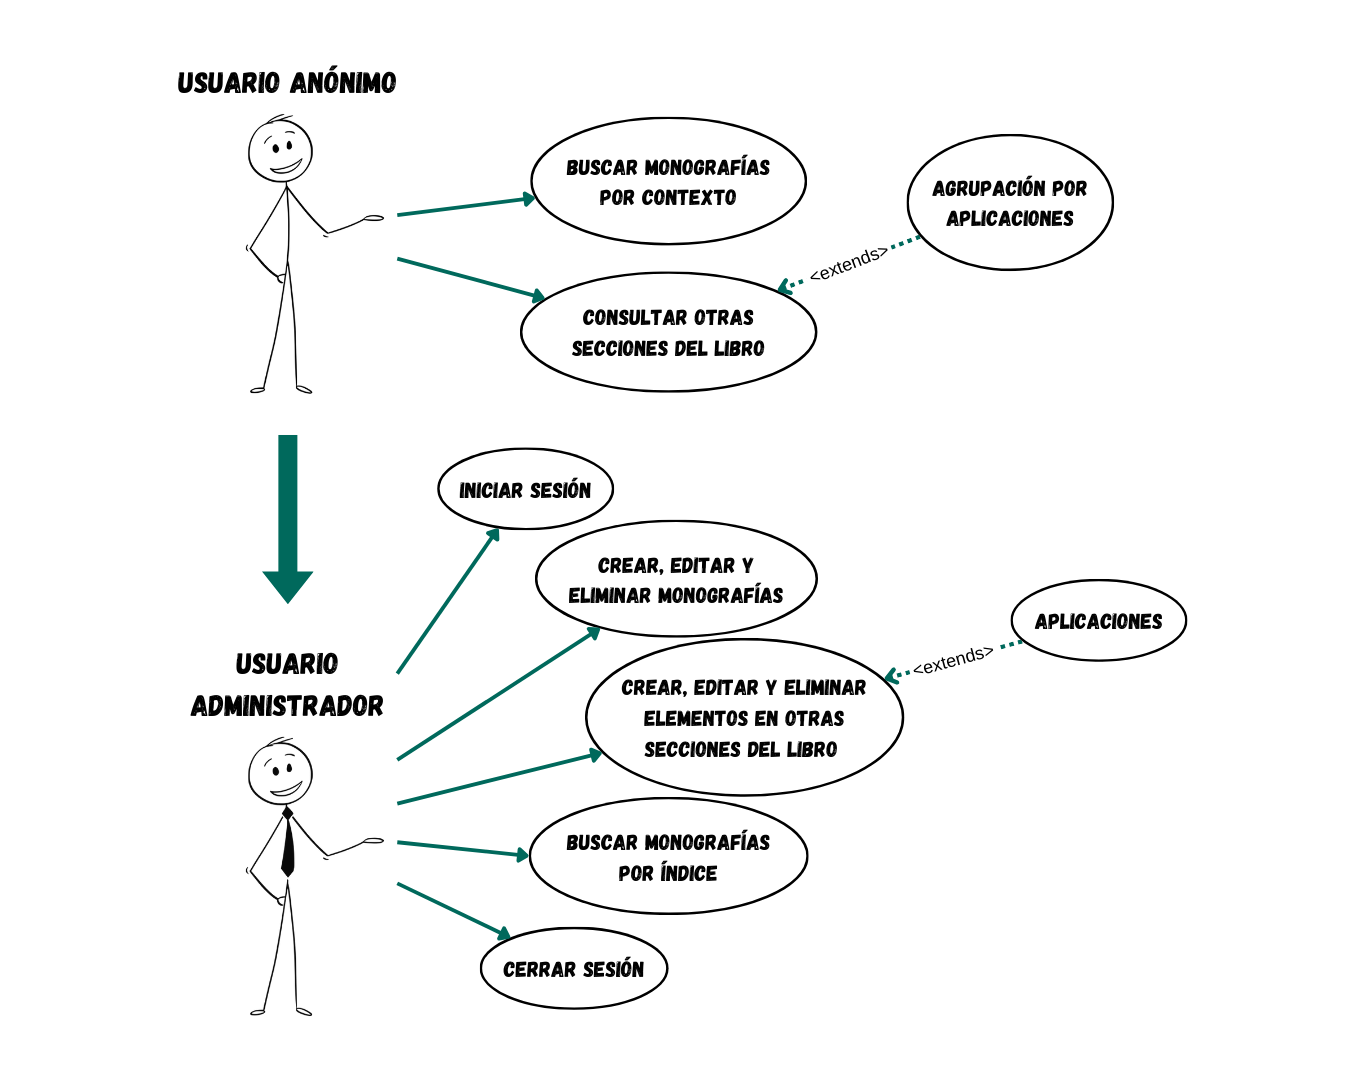
\includegraphics[width=0.9\textwidth]{Images/use-cases.png}
    \caption{Diagrama de casos de uso}
    \label{fig:use-cases}
\end{figure}




\section{Diseño de la solución}
Es posible identificar dos subproblemas principales dentro del contexto del problema anteriormente descrito mediante requerimientos. 
Estos subproblemas están interrelacionados y son fundamentales para garantizar que el sistema cumpla 
con los objetivos establecidos:

\begin{itemize}
    \item \textbf{Problema de la extracción de la información}: Este subproblema se refiere al proceso 
    de extraer, estructurar y almacenar de manera eficiente la información contenida en el libro de Tomás Roig, 
    de forma que estos datos puedan ser consumidos por un software computacional.
    \item \textbf{Problema del sistema de gestión y visualización de la información}: Una vez 
    extraída y estructurada la información, surge el desafío de diseñar e implementar un sistema que permita 
    gestionar y visualizar eficientemente los datos.
\end{itemize}

Esta sección tiene como objetivo presentar las estrategias y propuestas de diseño abstracto desarrolladas 
para abordar los subproblemas identificados anteriormente. 
Estos subproblemas, requieren soluciones específicas que garanticen tanto 
la fidelidad de los datos extraídos como su presentación efectiva a los usuarios finales.

En esta sección, se describirán los enfoques conceptuales diseñados para resolver cada 
uno de los subproblemas, teniendo en cuenta los requerimientos funcionales previamente establecidos. 
Se analizarán las características principales de cada solución, incluyendo sus componentes clave y cómo 
estos se integran para formar un sistema coherente y eficiente. Este análisis establecerá las bases 
para la implementación detallada del sistema.


\subsection{Extracción de la información}
Una solución al problema planteado debe partir de un análisis exhaustivo del corpus sobre el cual se 
realizará la extracción de información. En este sentido, tras examinar detalladamente el libro 
\textit{``Plantas medicinales, aromáticas o venenosas de Cuba''}, se identificaron una serie de observaciones 
preliminares. Estas observaciones constituyen la base para tomar decisiones informadas respecto 
a las estrategias de extracción de información que sean adecuadas y acordes con el estado del arte.

Las observaciones identificadas son las siguientes:
\begin{enumerate}
    \item La obra está dividida en dos tomos, por lo que es deseable que la solución adoptada sea 
    lo más general posible, permitiendo su aplicación efectiva en ambos tomos.
    \item Ambos tomos se encuentran en el formato: \textit{Portable Document Format} (PDF)
    \item Aunque pertenecen a la misma editorial, existen diferencias significativas 
    en cuanto a la maquetación y el diseño digital entre ambos tomos.
    \item Las monografías constituyen la sección fundamental del libro.
    \item El tomo 1 contiene las monografías de las plantas cuyos nombres inician con las letras de 
    la `A' a la `K', mientras que el tomo 2 abarca aquellas cuyas iniciales están entre la `L' y la `Z'.
    \item En las monografías se pueden identificar secciones principales que contienen cierta información 
    sobre las plantas. Estas secciones mantienen un orden fijo, aunque no siempre están 
    presentes todas en cada monografía. Las secciones identificadas son:
    \begin{itemize}
        \item Nombre con que se conoce la plantas.
        \item Nombre científico.
        \item Sinónimos.
        \item Otros nombres vulgares asociados.
        \item Hábitat y distribución geográfica.
        \item Descripción botánica.
        \item Composición química.
        \item Partes empleadas.
        \item Propiedades medicinales.
        \item Aplicaciones.
        \item Cultivo.
        \item Referencias bibliográficas.
    \end{itemize}
    \item Algunas monografías incluyen imágenes de baja calidad de las plantas, 
    acompañadas de un pie de foto que identifica el nombre de la especie.
    \item El formato de presentación del texto no es uniforme, lo que responde a decisiones editoriales y 
    de diseño. Por ejemplo, las monografías están dispuestas en una sola columna para facilitar la lectura continua, 
    mientras que otras secciones como la dedicada a la agrupación de plantas según sus aplicaciones 
    están organizadas en tres columnas para optimizar el uso del espacio al listar múltiples nombres.
\end{enumerate}

Estas características del corpus son consideradas para garantizar que la solución propuesta sea capaz de 
abordar los retos específicos que plantea la extracción de información en un contexto tan heterogéneo.

Es factible realizar la extracción del texto contenido en los documentos en formato \textit{PDF} mediante el uso 
de lenguajes de programación modernos, apoyándose en bibliotecas especializadas para la manipulación y 
el procesamiento de este tipo de archivos. No obstante, debe considerarse que el texto presenta 
características de maquetación no uniformes a lo largo de la obra, lo que podría requerir un manejo 
cuidadoso de las estructuras y formatos para asegurar una extracción precisa y completa.

En la sección \ref{section: nlp} se describe el problema general de la IE, identificándola como una 
de las tareas más comunes y relevantes en el ámbito del Procesamiento del NLP. La IE
se enfoca en identificar, estructurar y representar conocimiento relevante a partir de 
textos no estructurados o semiestructurados.

Dadas las características del corpus objeto de estudio y su estructura textual, la técnica seleccionada 
para llevar a cabo el proceso de extracción de información es la denominada \textit{template filling} abordada en la sección \ref{section: templateFilling}. 
Esta técnica permite extraer información específica mediante la identificación de patrones 
predefinidos y su mapeo en plantillas estructuradas. La elección de esta metodología 
responde a varios factores:
\begin{enumerate}
    \item La necesidad de obtener los datos en un formato estructurado que facilite su posterior uso
    en sistemas computacionales.
    \item La importancia de preservar las palabras y expresiones originales del autor 
    para garantizar una representación precisa del contenido de la obra.
    \item La adecuación de esta técnica para procesar textos con una organización semiuniforme, 
    como las monografías presentes en la obra, permitiendo capturar información clave como 
    nombres científicos, descripciones botánicas, propiedades y aplicaciones.
\end{enumerate}

Para mayor conveniencia, se optará por realizar la extracción de información del libro de manera segmentada, 
abordando cada sección de forma independiente. Este enfoque permite aplicar el proceso de \textit{template filling} 
a cada sección por separado, lo cual simplifica significativamente los algoritmos necesarios para la extracción.



\subsubsection{Template Filling en monografías}
Para la extracción de información de las monografías, se optará por un enfoque basado en reglas, 
considerando las características semiestructuradas de los datos presentes en esta sección del libro. 
El diseño de la plantilla requerirá abordar tres aspectos fundamentales: la definición 
de la estructura de la plantilla, la especificación de las reglas de interpretación 
y la documentación de casos. Sin embargo, este último punto no será desarrollado, 
dado que su utilidad sería limitada en ausencia de un enfoque basado en aprendizaje automático.

En una etapa inicial, es posible extraer la información correspondiente a cada monografía 
de manera básica. Esto implica definir una plantilla inicial que incluya los nombres de 
todas las plantas mencionadas en el libro, asociando a cada nombre el texto plano que 
representa la información respectiva. La regla de interpretación empleada en este paso se 
encargará de identificar el inicio de cada monografía, utilizando como criterio el nombre de 
la planta, que se encuentra destacado con un tamaño de fuente significativo en el texto.

A partir de esta extracción inicial, se procederá a estructurar la información de cada monografía 
basándose en su contenido. En la Figura \ref{fig:template-monograph}, se presenta la definición de la plantilla utilizada 
para este propósito, en la que se incluye el nombre de cada atributo, junto con el tipo de dato del mismo.

\begin{figure}[ht!]
    \centering
    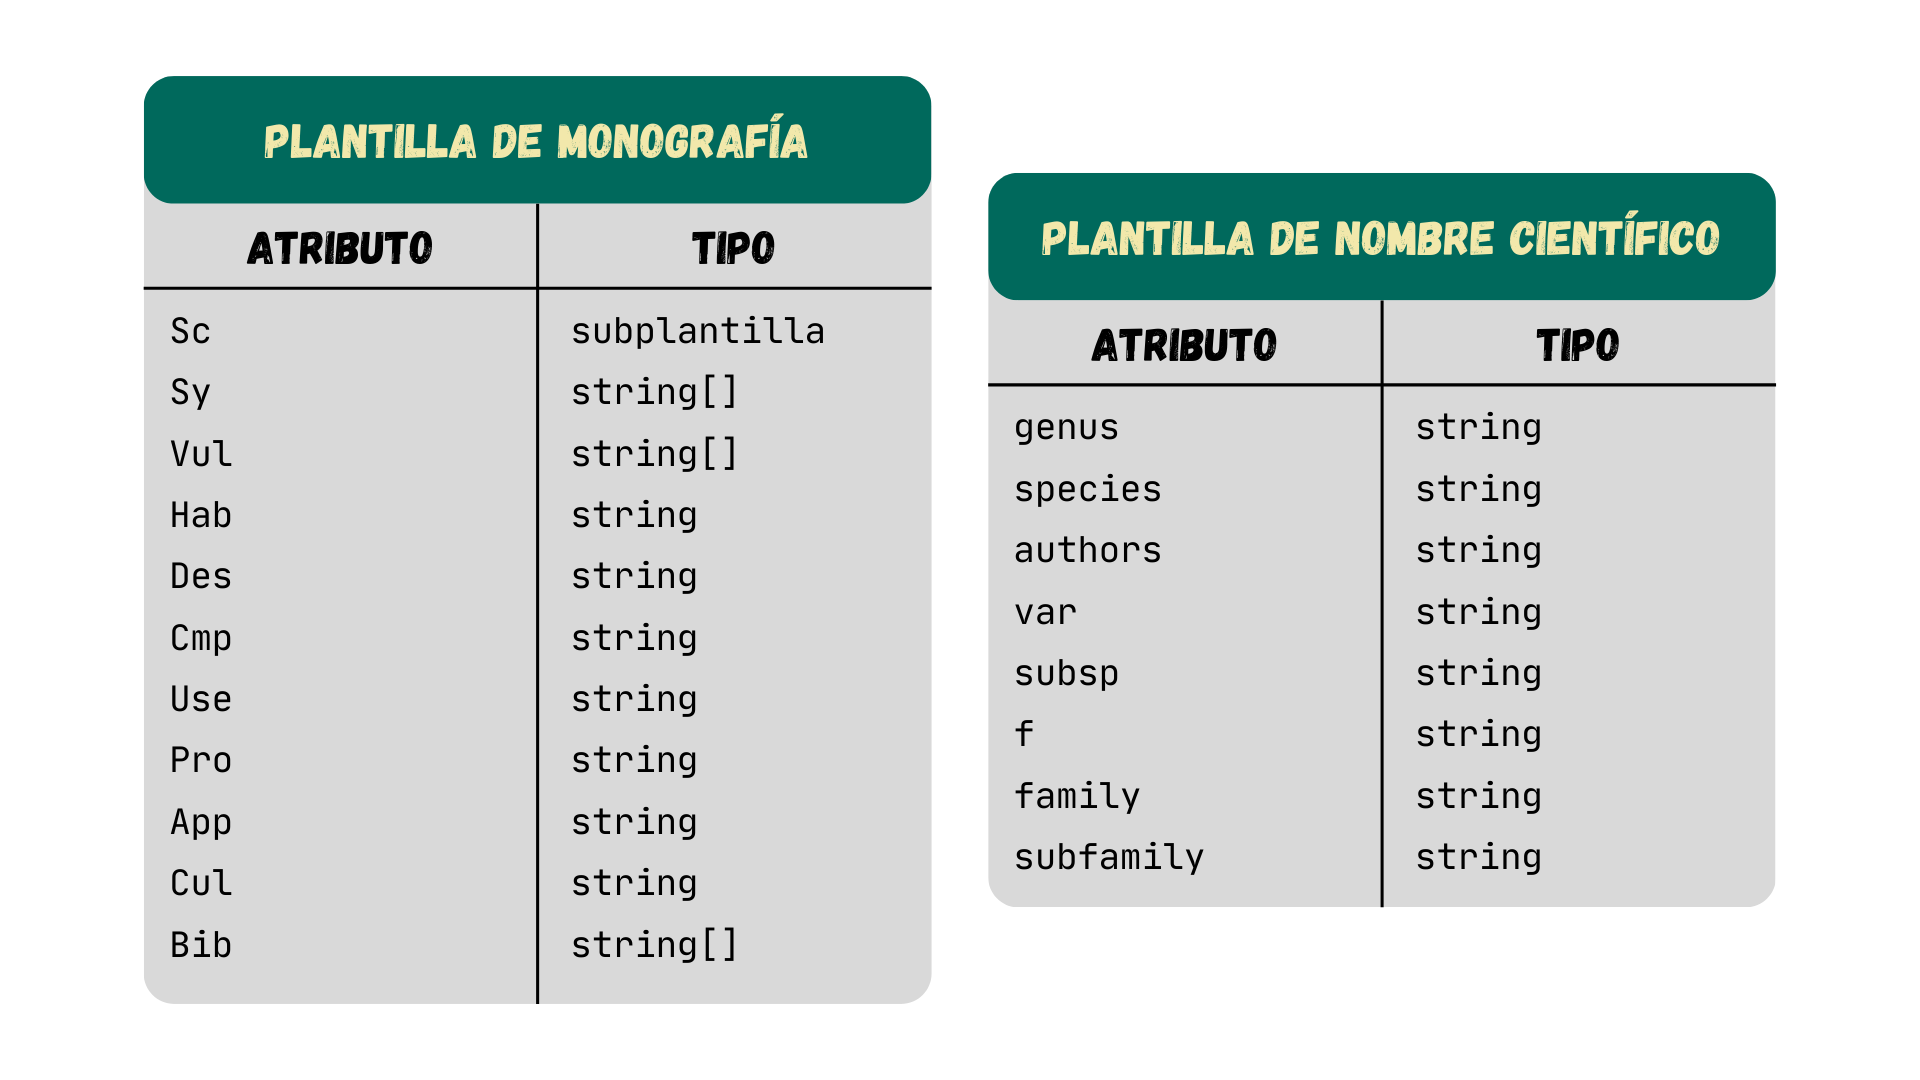
\includegraphics[width=1\textwidth]{Images/monograph-template.png}
    \caption{Plantillas de monografía y nombre científico}
    \label{fig:template-monograph}
\end{figure}

Cada atributo de la plantilla corresponde a una sección identificable dentro del contenido 
de una monografía. Por ejemplo, 
\texttt{Sc} representa el nombre científico, 
\texttt{Sy} los sinónimos,
\texttt{Vul} los nombres vulgares asociados, 
\texttt{Hab} el hábitat y distribución geográfica, 
\texttt{Des} la descripción botánica, 
\texttt{Cmp} la composición química, 
\texttt{Use} las partes empleadas, 
\texttt{Pro} las propiedades medicinales, 
\texttt{App} las aplicaciones, 
\texttt{Cul} el cultivo y 
\texttt{Bib} las referencias bibliográficas.

Como se observa en la Figura \ref{fig:template-monograph}, este diseño emplea una plantilla híbrida 
que combina características de plantillas planas y plantillas orientadas a objetos, 
permitiendo que los atributos puedan almacenar tanto datos primitivos como subplantillas, 
lo que facilita una representación más estructurada y flexible de la información.

Definamos entonces las reglas de interpretación para la plantilla de las monografías:
\begin{enumerate}
    \item Las secciones dentro de una monografía siempre aparecen en el mismo orden, y no necesariamente aparecen todas en una monografía.
    \item El nombre científico siempre aparece en la primera línea inmediatamente después del título de la monografía.
    \item Los sinónimos están precedidos por la cadena de texto \texttt{``SINÓNIMOS:''} y se encuentran separados entre sí por comas (\texttt{,}).
    \item Los otros nombres vulgares están precedidos por la cadena de texto \texttt{``OTROS NOMBRES VULGARES:''}. Los nombres correspondientes a un mismo territorio están separados por comas (\texttt{,}), mientras que los nombres entre territorios están separados por punto y coma (\texttt{;}).
    \item El texto correspondiente al hábitat y distribución está precedido por la cadena de texto \texttt{``HÁBITAT Y DISTRIBUCIÓN:''}.
    \item El texto correspondiente a la descripción botánica está precedido por la cadena de texto \texttt{``DESCRIPCIÓN BOTÁNICA:''}.
    \item El texto correspondiente a la composición química está precedido por la cadena de texto \texttt{``COMPOSICIÓN:''}.
    \item El texto correspondiente a las partes empleadas está precedido por la cadena de texto \texttt{``PARTES EMPLEADAS:''}.
    \item El texto correspondiente a las propiedades de la planta está precedido por la cadena de texto \texttt{``PROPIEDADES:''}.
    \item El texto correspondiente a las aplicaciones está precedido por la cadena de texto \texttt{``APLICACIONES:''}.
    \item El texto correspondiente al cultivo de la planta está precedido por la cadena de texto \texttt{``CULTIVO:''}.
    \item El texto correspondiente a las referencias bibliográficas está precedido por la cadena de texto \texttt{``BIBLIOGRAFÍA''}, y cada bibliografía termina en el año correspondiente a la misma.
\end{enumerate}

En cuanto a los nombres científicos, se pueden definir las siguientes reglas en función de la plantilla:
\begin{enumerate}
    \item Las partes que componen un nombre científico siempre siguen un orden específico, aunque no necesariamente todas deben estar presentes.
    \item Las primeras dos palabras corresponden al género y la especie, respectivamente.
    \item La autoridad de la planta siempre aparece inmediatamente después del género y la especie.
    \item La variedad siempre está precedida por la cadena de texto \texttt{``var.''}.
    \item La subespecie siempre está precedida por la cadena de texto \texttt{``subsp.''}.
    \item La forma siempre está precedida por la cadena de texto \texttt{``f.''}.
    \item La familia siempre está precedida por la cadena de texto \texttt{``Fam.''}.
    \item La subfamilia siempre está precedida por la cadena de texto \texttt{``Subfam.''}.
\end{enumerate}

Con la definición de estas plantillas y reglas de interpretación, se logra un diseño adecuado para 
la extracción de la información de las monografías, asegurando que los datos sean identificados y 
estructurados correctamente de acuerdo con su formato original.


\subsubsection{Template Filling en agrupación de plantas por aplicaciones}
La sección del libro que agrupa las plantas según sus aplicaciones se presenta con un diseño de 
tres columnas, optimizado para maximizar el uso del espacio disponible. En consecuencia, será 
necesario realizar una lectura ordenada que permita obtener el texto plano de toda la sección, 
a fin de aplicar la técnica de \textit{template filling}.

De manera análoga a lo realizado en la sección de las monografías, se empleará un enfoque basado 
en reglas para abordar esta sección del libro. Inicialmente, es posible identificar todas las aplicaciones 
mencionadas, bajo la regla de que los nombres de las aplicaciones aparecen completamente en mayúsculas y 
finalizan con el caracter de dos puntos (\texttt{:}), mientras que los nombres de las plantas contienen caracteres en minúsculas.
Esto nos lleva a tener una plantilla que tiene como atributos los nombres de todas las aplicaciones.

Al analizar la sección, se observa que algunas aplicaciones incluyen referencias a otras ya mencionadas, 
debido a que estas representan sinónimos o significados equivalentes. En estos casos, resulta útil que 
cada aplicación cuente con una lista de sinónimos que agrupe dichas referencias. Por lo tanto, se definirá 
una subplantilla como tipo de cada atributo en la plantilla anterior, adoptando la estructura ilustrada en 
la Figura \ref{fig:template-app}.

\begin{figure}[ht!]
    \centering
    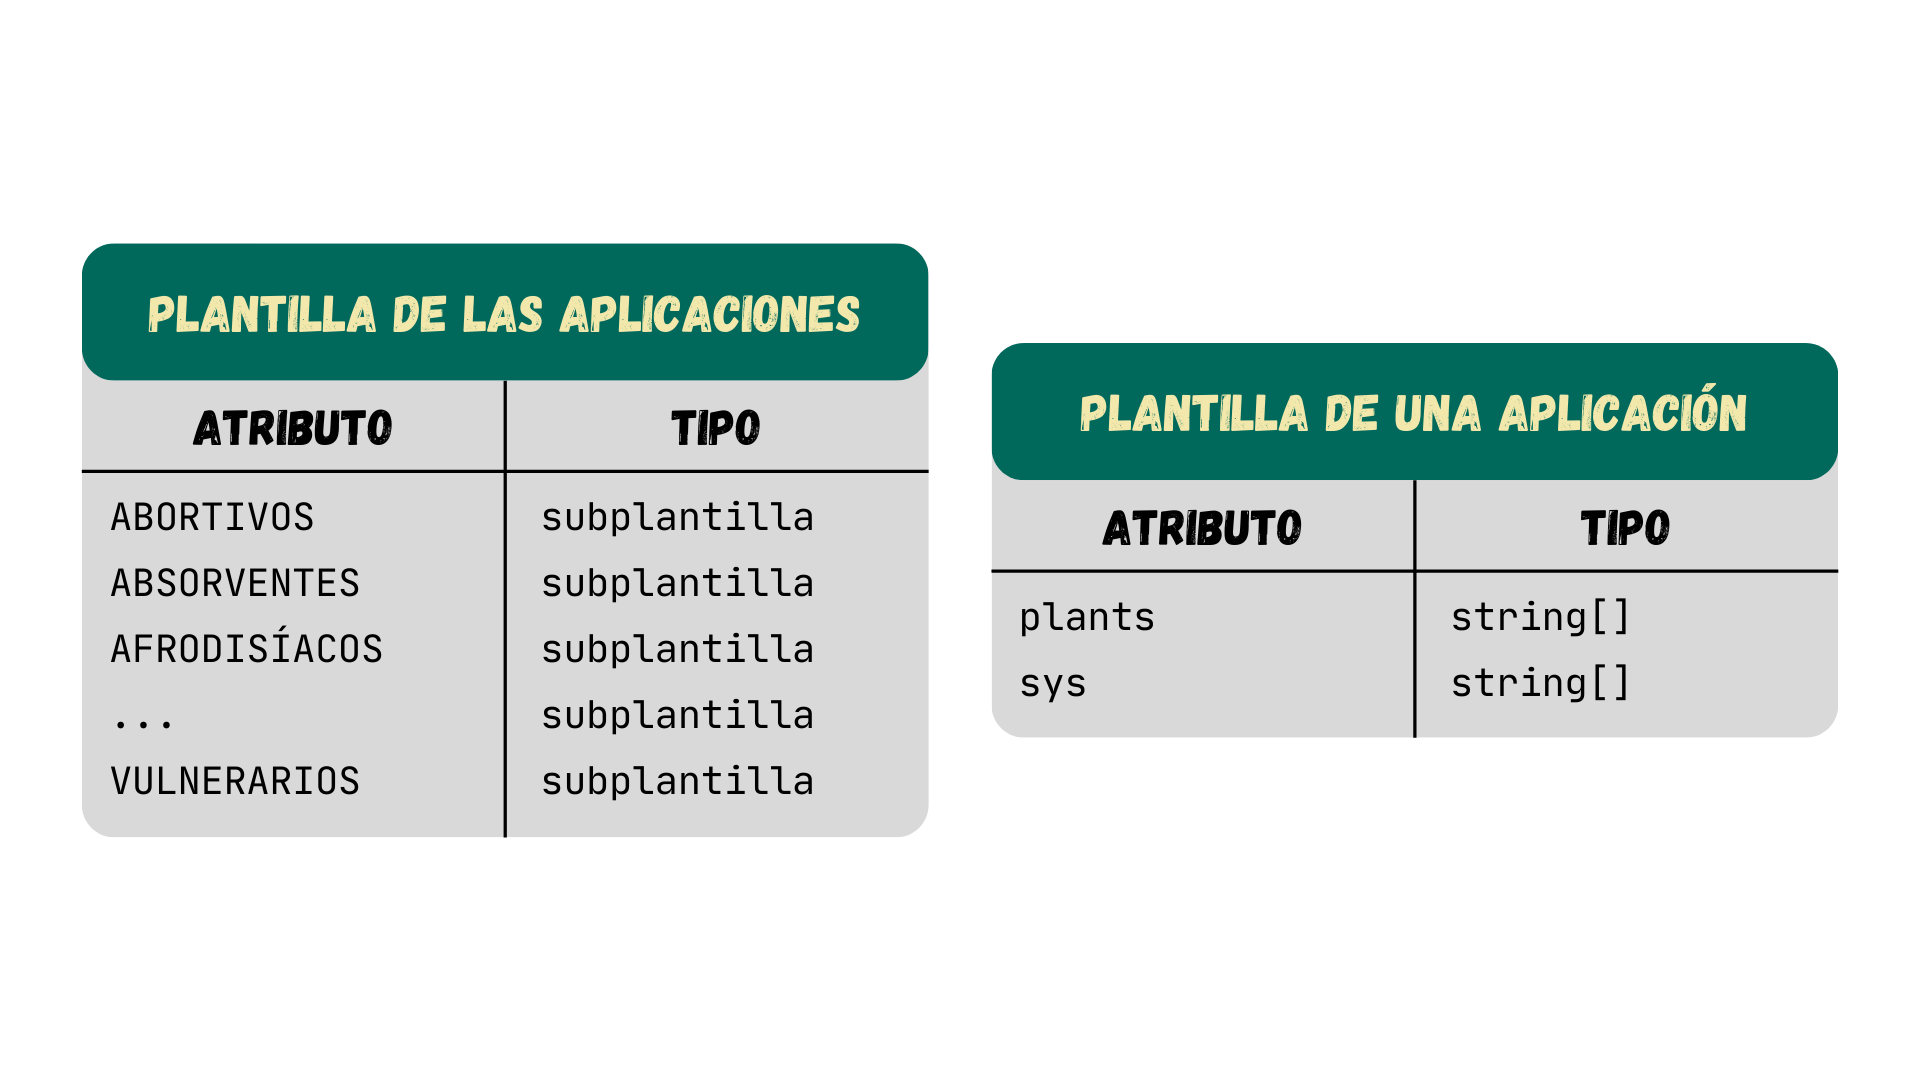
\includegraphics[width=1\textwidth]{Images/app-template.png}
    \caption{Plantillas de aplicaciones}
    \label{fig:template-app}
\end{figure}

Es posible observar que para cada aplicación tendremos una subplantilla que almacena dos listas, una con los nombres
de todas las plantas que tienen esa aplicación, y otra con los sinónimos identificados en el texto.

En base a lo anterior definimos las reglas de llenado:

\begin{enumerate}
    \item Las plantas asociadas a cada aplicación comienzan con el nombre de esta última, seguido por el caracter de dos puntos (\texttt{:}).
    \item En general, los nombres de las plantas se identifican por los saltos de línea, salvo en algunos casos excepcionales.
    \item Los casos excepcionales incluyen palabras que no caben en una misma línea, las cuales se indican mediante un guion (\texttt{-}), señalando que el nombre continúa en la siguiente línea.
    \item Algunas aplicaciones presentan, justo a continuación de su nombre, el nombre de otra aplicación entre paréntesis, lo que indica que heredan las plantas asociadas a esta última.
    \item Las referencias a otras aplicaciones se identifican por la cadena de caracteres \texttt{``Véase''}, seguida del nombre de la aplicación correspondiente.
\end{enumerate}




\subsection{Sistema de gestión y visualización}
El diseño de un sistema web eficiente y escalable requiere la separación clara entre el frontend y el backend, 
siguiendo los principios de modularidad y responsabilidad única. El frontend se ocupa de la presentación y 
experiencia del usuario, mientras que el backend se encarga de procesar la lógica del negocio, gestionar la 
persistencia de datos y exponer interfaces (APIs) para interactuar con el sistema. Este enfoque asegura que 
cada componente pueda desarrollarse, mantenerse y escalarse de manera independiente.

En el caso del backend, se empleará una arquitectura por capas que permita una separación clara de responsabilidades. 
Esta arquitectura incluirá las siguientes capas principales:

\begin{enumerate}
    \item \textbf{Capa de datos}: Responsable de modelar las entidades del dominio.
    \item \textbf{Capa de acceso a datos}: Proveerá métodos especializados para interactuar con la base de datos, 
    aislando las operaciones sobre la misma de la lógica de negocio.
    \item \textbf{Capa de servicios}: Implementará la lógica del negocio y las reglas del sistema, ofreciendo 
    funcionalidades como servicios que serán consumidos posteriormente.
\end{enumerate}

Estas capas estarán integradas en un proyecto principal de backend, cuya función será consumir los servicios para exponer una serie de APIs 
que sirvan como puente entre los frontends y la lógica del sistema. Este diseño por capas garantiza mantenibilidad, 
escalabilidad y reutilización del código.

Debido a los requerimientos del sistema, se necesitarán dos módulos principales: un módulo de administración y 
un módulo orientado al cliente final de internet. Cada uno de estos módulos contará con un proyecto independiente 
de frontend para cubrir las necesidades específicas de cada tipo de usuario. Este enfoque asegura que ambos 
módulos sean autónomos en su desarrollo y despliegue, al tiempo que se preserva la consistencia general del sistema.

Para optimizar el uso de recursos y evitar redundancias, las capas de datos, acceso a datos y servicios del backend 
serán compartidas entre los módulos. Esto significa que, aunque se desarrollen dos proyectos de web API 
(uno para el módulo de administración y otro para el cliente final), ambos consumirán las mismas capas internas de 
lógica y acceso a datos. De esta manera, se centraliza la lógica común en un solo lugar, promoviendo la 
reutilización del código, simplificando el mantenimiento y facilitando la escalabilidad del sistema ante posibles 
cambios o nuevas funcionalidades en el futuro. En la Figura \ref{fig:architecture} se ilustra la arquitectura explicada del sistema.

\begin{figure}[ht!]
    \centering
    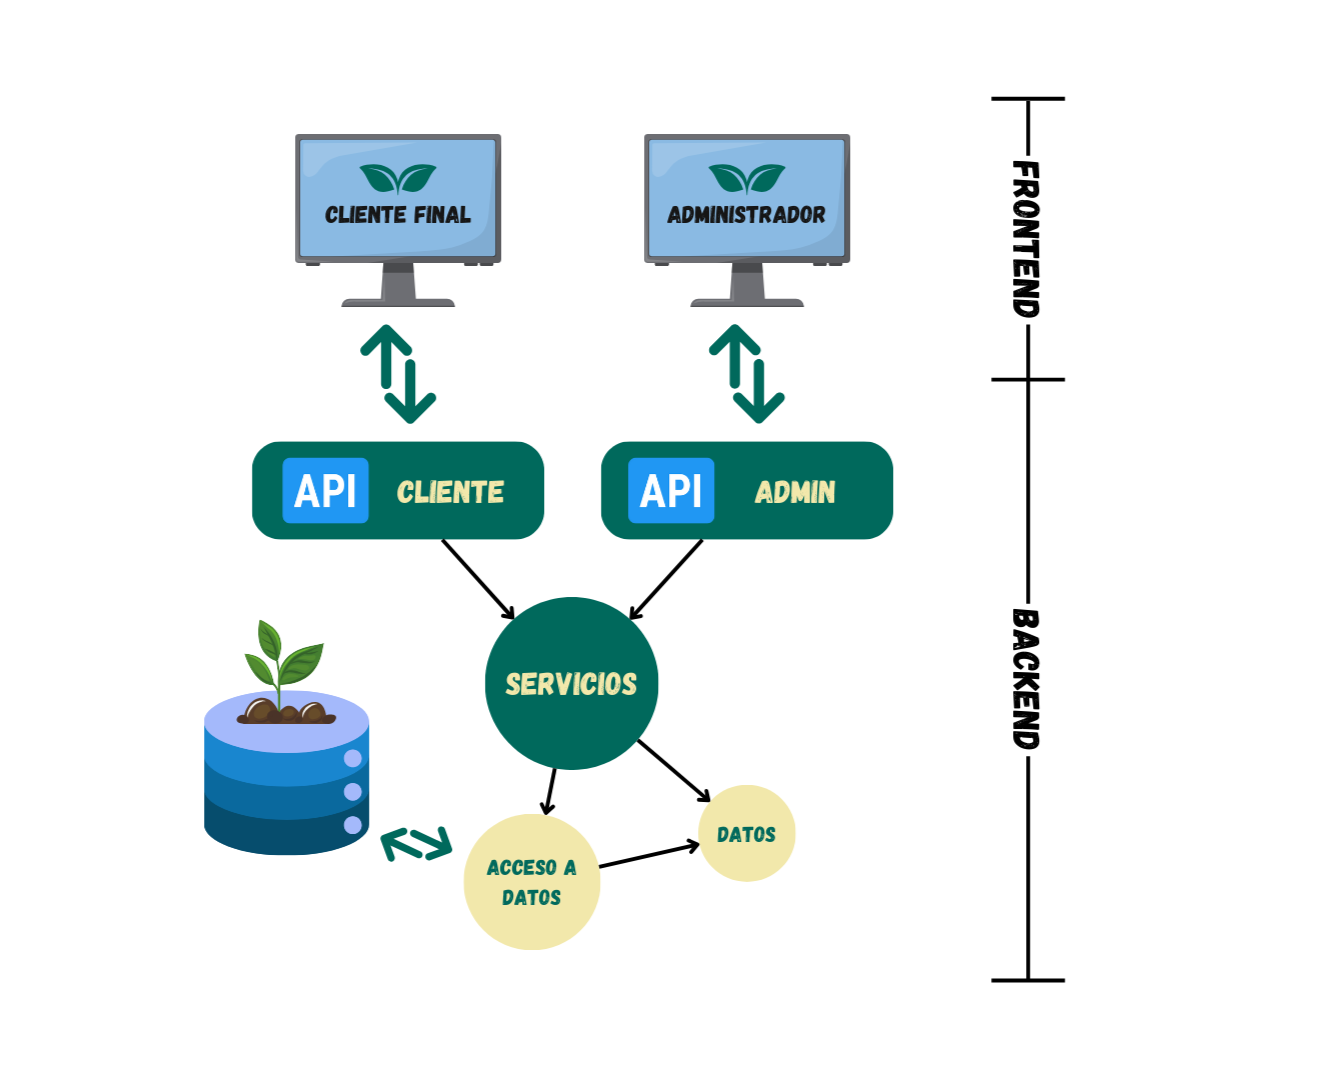
\includegraphics[width=0.9\textwidth]{Images/architecture.png}
    \caption{Arquitectura del sistema}
    \label{fig:architecture}
\end{figure}


En el módulo de administración, será necesario implementar servicios específicamente dirigidos a la gestión de 
los recursos almacenados en el sistema, lo cual resulta inherente a su propósito. Estos servicios permitirán 
realizar las operaciones fundamentales sobre entidades que conforman los datos. Entre estas operaciones se incluyen 
la creación de nuevos registros, la consulta de información existente, la actualización de datos 
según sea necesario y la eliminación de registros obsoletos o irrelevantes. Este conjunto de funcionalidades, 
comúnmente denominadas operaciones de mantenimiento de datos, garantizará que el administrador tenga un 
control total sobre el contenido y pueda gestionar de manera eficiente la información que se ofrece en el sistema.

Estas operaciones serán esenciales para mantener actualizados y organizados los datos, y asegurar la consistencia y 
la calidad de la información. Además, al centralizar estos servicios en el módulo de administración, se logra una 
clara separación entre las funcionalidades destinadas al mantenimiento interno del sistema y aquellas orientadas 
al usuario final, promoviendo una mayor modularidad, escalabilidad y orden en el diseño.

Adicionalmente, el sistema contará con un método de autenticación dedicado específicamente al usuario administrador. 
Este mecanismo de seguridad será fundamental para garantizar que solo usuarios autorizados puedan acceder a las herramientas 
de gestión. La implementación de esta autenticación asegura el resguardo de los datos almacenados, y la integridad 
del sistema, permitiendo que las operaciones de mantenimiento se lleven a cabo de manera controlada y segura.


El sistema contará con un método avanzado de búsqueda diseñado para que los usuarios puedan localizar de manera eficiente y 
precisa las plantas disponibles en la plataforma. Este método estará basado en el Modelo de Espacio Vectorial, una técnica 
ampliamente utilizada en el campo de la IR por su capacidad para manejar grandes volúmenes de datos textuales. 
Este modelo representa los datos como vectores en un espacio multidimensional, donde cada dimensión corresponde a términos 
relevantes en las descripciones de las plantas. Dada la naturaleza textual y extensa de las monografías y la cantidad 
significativa de información almacenada, este enfoque resulta especialmente adecuado, ya que permite gestionar y 
procesar el contenido de manera eficiente.

El Modelo de Espacio Vectorial posibilitará una búsqueda por contexto, lo que significa que el sistema no se limitará a 
buscar coincidencias exactas de palabras, sino que también identificará resultados relevantes en función de la relación 
semántica entre las palabras utilizadas en la consulta y las descripciones de las plantas. Por ejemplo, si un usuario 
busca una planta por sus propiedades medicinales o sus características, el sistema podrá identificar plantas relacionadas 
incluso si las palabras exactas no coinciden, mejorando así la experiencia de búsqueda.

La implementación de este modelo busca ofrecer una herramienta poderosa y flexible que permita a los usuarios acceder 
de manera intuitiva a la información científica almacenada, respondiendo a sus necesidades de una forma rápida, 
precisa y relevante. Esta debe ser una funcionalidad clave del sistema, que facilitará la navegación por el contenido 
y potenciará su utilidad para diversos tipos de usuarios, desde investigadores hasta profesionales de la salud y 
el público general.


\subsubsection{El modelo de datos}
El modelo de datos proporciona la estructura necesaria para almacenar, gestionar y acceder de manera eficiente a la información. 
Basado en las entidades fundamentales del dominio, el modelo representa los elementos clave que se gestionarán a lo largo de su 
ciclo de vida, estableciendo relaciones entre ellos. Es esencial que el diseño de estas relaciones esté bien estructurado, 
alineado con los requerimientos funcionales y las características del sistema, para garantizar la alta integridad y disponibilidad 
de los datos, así como para facilitar las consultas y optimizar el rendimiento del sistema.

Los principales componentes del modelo de datos son:

\begin{enumerate} 
    \item \textbf{Entidades del dominio}: Son los objetos principales con los que interactuarán los usuarios y el sistema. 
    En nuestro caso, estas entidades incluirán elementos como plantas, términos, aplicaciones y usuarios. Cada entidad se representará 
    por una tabla en la base de datos, y sus atributos corresponden a las columnas de dichas tablas.
    \item \textbf{Relaciones entre entidades}: Las entidades no operan de manera aislada, sino que se interconectan entre sí. Las relaciones 
    entre las entidades pueden ser de uno a uno, uno a muchos o muchos a muchos, y deben estar modeladas adecuadamente en el esquema de la 
    base de datos. Estas relaciones permiten que los datos sean accesibles y actualizados de manera coherente en todo el sistema.
    \item \textbf{Normalización y optimización}: Para garantizar la eficiencia en el acceso y la integridad de los datos, se llevará a cabo un 
    proceso de normalización. La normalización busca reducir la redundancia de los datos y mejorar la consistencia de las relaciones. Esto significa 
    que cada tipo de información debe estar en su lugar adecuado, sin duplicar datos innecesarios.
    Además, se implementarán índices y claves foráneas para optimizar las consultas y mantener la integridad referencial.
    \item \textbf{Persistencia de datos}: El modelo de datos se implementará utilizando herramientas que permitan almacenar, consultar y actualizar la información de manera eficiente.
\end{enumerate}

El modelo de datos será la base sobre la cual se construirán los servicios y las APIs del sistema. Cada operación o servicio del backend interactuará con la base de datos a través 
de las capas de acceso a datos y servicios, garantizando que las transacciones sean consistentes y eficaces.

Aunque el carácter variable de las secciones presentes en las monografías podría sugerir el uso de una base de datos NoSQL, se optará por utilizar una base de datos relacional (SQL).
Esta decisión de emplear SQL está motivada por el enfoque adoptado en el diseño, donde se utiliza un modelo basado en plantillas estructuradas para representar la información de las monografías.
Sin embargo es importante destacar la utilidad que pudiesen otorgar las características de las bases de datos NoSql.

% Además, se basa en las capacidades avanzadas de \textbf{PostgreSQL}, que, a pesar de ser una base de datos relacional, ofrece soporte nativo para el almacenamiento de datos semi-estructurados 
% mediante los tipos de datos \textbf{JSON} y \textbf{ARRAY}. 

% El modelo de relaciones se adaptará a un enfoque flexible mediante el uso de \textbf{JSON} para almacenar las secciones de las monografías, facilitando así la devolución de los datos en un formato 
% directamente utilizable por aplicaciones y servicios, sin necesidad de realizar transformaciones adicionales. Dado que muchas aplicaciones modernas, como las interfaces web, 
% consumen y manipulan datos en formato \texttt{JSON}, este enfoque permitirá una integración más eficiente, proporcionando una respuesta cómoda y rápida.

Se busca concebir un enfoque que permita adaptar el modelo de relaciones a una estructura más flexible, orientada a simplificar el acceso y procesamiento de los datos almacenados. 
Este diseño aspira a minimizar operaciones costosas dentro de la base de datos, con el objetivo de ofrecer una respuesta más directa y eficiente a las aplicaciones y servicios que 
consumen la información. Al reducir la necesidad de transformaciones adicionales, se espera que la solución facilite la integración con otros sistemas y optimice los tiempos de respuesta, 
promoviendo una experiencia más ágil y fluida.

% Los vectores \textbf{TF-IDF}, que representan la 
% importancia de los términos en las monografías, se almacenarán como \textbf{arrays}, lo que facilitará las operaciones de búsqueda y cálculo de similitudes. Este enfoque no solo 
% aprovecha la flexibilidad que caracteriza a las bases de datos NoSQL, sino que también mantiene las fortalezas del modelo relacional, como las consultas optimizadas y la integridad de los datos.

Los vectores \textbf{TF-IDF} que utiliza el Modelo de Espacio Vectorial, y que representan la importancia de los términos en las monografías, se deben gestionar de manera que 
faciliten las operaciones de búsqueda y cálculo de similitudes. Un enfoque así aprovechará las ventajas de un sistema de bases de datos SQL, manteniendo la flexibilidad necesaria 
para realizar consultas eficientes y garantizando la integridad de los datos.

El modelo de relaciones se basará en un enfoque de muchos a muchos entre las entidades Planta y Término (a través de PlantTerm), así como entre Planta y Aplicación (a través de PlantApp). 
Estas relaciones intermedias permitirán flexibilidad en el sistema, permitiendo que cada planta esté asociada a múltiples términos y aplicaciones y viceversa, y de esta forma mantener la integridad 
referencial y evitar problemas de redundancia. 

En el caso de la entidad Usuario, no se encontrará interrelacionada directamente con las demás entidades, siendo completamente autónoma, lo que simplifica su manejo y permite 
que los usuarios interactúen con el sistema sin necesidad de relaciones directas con las demás entidades del dominio.

Para facilitar la comprensión de la estructura de la base de datos, el diagrama de la Figura \ref{fig:merx} ilustra el Modelo Entidad-Relación-Extendido (MERX) del sistema, que refleja las entidades principales y sus relaciones clave.

\begin{figure}[ht!]
    \centering
    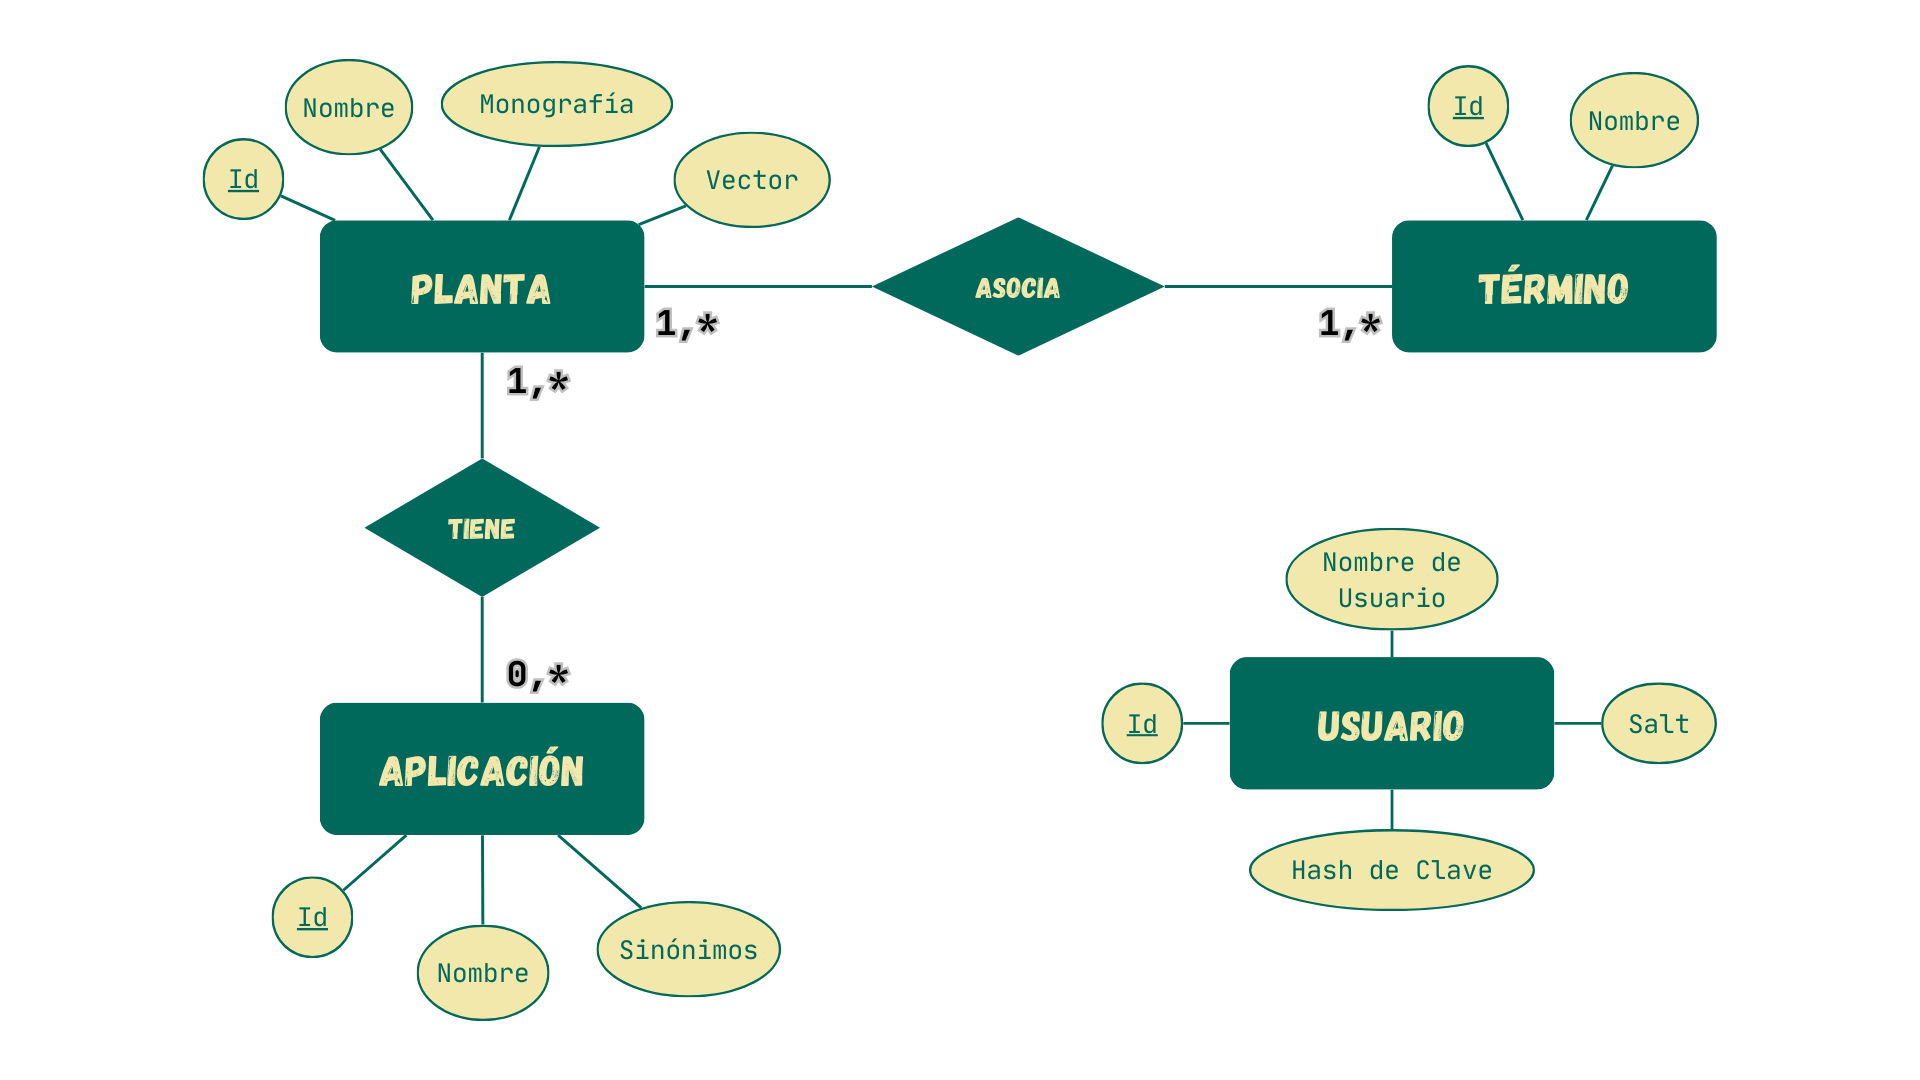
\includegraphics[width=0.9\textwidth]{Images/merx_es.png}
    \caption{MERX}
    \label{fig:merx}
\end{figure}
